\documentclass{article}
\usepackage[UTF8]{ctex}
\usepackage{tikz}
\usepackage[tc]{titlepic}
\usepackage{titlesec}
\usepackage{cite}
\usepackage{fancyhdr}
\usepackage{booktabs}
\usepackage{graphicx}
\usepackage{subfigure} 
\usepackage{geometry}
\usepackage{amsmath}
\usepackage[section]{placeins}
\geometry{a4paper,scale=0.8}
\pagestyle{fancy}

\lhead{第 3 次作业\\\today}
\chead{中国科学技术大学\\数学建模课程}

\rhead{Assignment 3\\ {\CTEXoptions[today=old]\today}}
\newcommand{\upcite}[1]{\textsuperscript{\cite{#1}}}

\titleformat*{\section}{\bfseries\Large}
\titleformat*{\subsection}{\bfseries\large}

\title{\bfseries 作业3 神经网络模型}
\author{晏瑞然 \quad  87 \quad  PB19000196}

\begin{document}
\maketitle
\begin{abstract}
    通过简单的神经网络(Neural Networks)模型,得到一个分类器,实现对昆虫以及一个20类点集的分类。
\end{abstract}
\newpage
% \setcounter{secnumdepth}{1}
 \setcounter{section}{1}
\section*{\centerline{一、前言}}
\subsection{神经网络介绍}
模拟人类实际神经网络的数学方法问世以来,人们已慢慢习惯了把这种人工神经网络直接称为神经网络。神经网络在系统辨识、模式识别、智能控制等领域有着广泛而吸引人的前景,特别在智能控制中,人们对神经网络的自学习功能尤其感兴趣,并且把神经网络这一重要特点看作是解决自动控制中控制器适应能力这个难题的关键钥匙之一。  \\
\subsection{问题概述}
有两组数据——训练集(training set)与测试集(test set),训练集包含元素的特征(features)与标签(labels),测试集只有元素的特征。构造一个神经网络并通过训练集训练神经网络模型,使之能够预测测试集中元素的标签。 
 \setcounter{section}{2}
\section*{\centerline{二、相关工作}}
    引用文献\upcite{0Learning}
 \setcounter{section}{3}
\section*{\centerline{三、问题分析}}
​		不妨设特征的个数为m,需要分的类的个数为n。所谓的分类,即找到一个m维到n维的映射$f:R^m\rightarrow R^n$ ,通过该映射便能将特征映射成标签。

​		要通过训练集得到这个映射,首先的构造一个网络,每层的神经元由上一层所有神经元映射而来,第一层神经元就是特征,最后一层即为得到的标签。隐藏层的神经元代表着特征中的隐藏的特征,最终输出我们需要的隐藏特征,即元素标签。

​		神经元之间的映射首先想到的便是用线性组合,但这并不好,如果只有线性组合那么整个网络都只有特征的线性相关项,那么整个网络就没有意义只不过是一个线性映射,这在一些数据集非线性分类的情况下会失去意义,如一个分类标准是一个圆,圆内为labe[0]圆外为label[1],这种方法就会失效。所以我们需要在映射中加入非线性项,我们就在线性映射上加一个激活函数,激活函数的种类有很多,如relu函数,softmax函数…通过这些非线性函数对网络加入非线性项,使得网络能够非类非线性模型。

​		网络的训练通过反向传播BP(back propagation)算法,不断修改网络层中的线性映射的系数,最终便能得到想要的映射。

\newpage
 \setcounter{subsection}{0}
 \setcounter{section}{4}
\section*{\centerline{四、建模的假设}}
    \subsection{假设1}
    所给数据集是可分的,可以有噪声但不能不可分。
    \subsection{假设2}
    所有数据不能有特征相同但标签不同的情况。
 
 
 \setcounter{section}{5}
 \section*{\centerline{五、符号说明}}

 \begin{table}[htbp]
    \caption{\textbf{符号说明}}%标题
    \centering%把表居中
    \begin{tabular}{ccc}%内容全部居中
    \toprule%第一道横线
    符号&说明 \\
    \midrule%第二道横线 
    $x_i$ & 第i个特征向量 \\
    $y_i$ & 第i个输出 \\
    $m$ & 特征的维度\\
    $n$ & 输出的维度\\
    $N$ & 总数据量\\
    $x_{ic}$ & 第i个特征向量的第c个特征 \\
    $y_{ic}$ & 1表示第i个数据标签是c,0反之 \\
    $p_{ic}$ & 第i个输出是第c类的概率 \\
    $X^{k}$ & 第k层神经元组成的列向量 \\
    $\omega_{ij}^{k}$ & k层网络i神经元到下层j神经元的权重\\
    $W^{k}$ & $\omega_{ij}^{k}$组成的系数矩阵\\
    $\alpha$ & 学习速率\\
    $b$ & bias项\\
    $act$ & 激活函数\\

    \bottomrule%第三道横线
    \end{tabular}
\end{table}

\newpage
\setcounter{subsection}{0}
 \setcounter{section}{6}
\section*{\centerline{六、数学模型建立}}
\subsection{神经网络}
\begin{center}

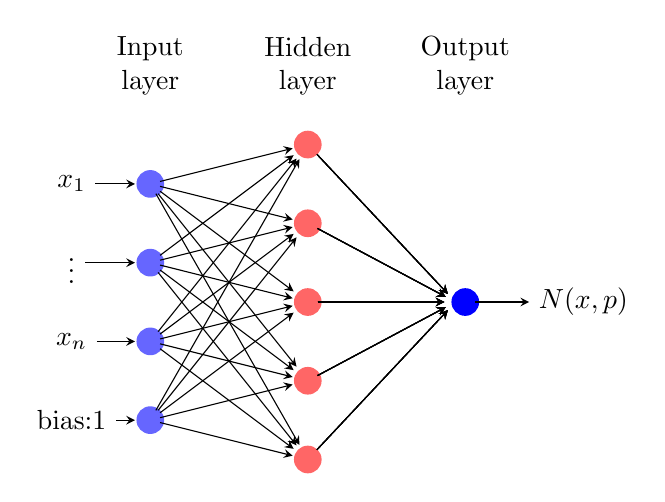
\begin{tikzpicture}[every node/.style={align=center}]
    \foreach \x in{1,2,3,4,5}
	\fill[red!60](0,\x)circle(5pt)node(a\x){};
	\fill[blue!60](-2,1.5)circle(5pt)node(b1){};
	\fill[blue!60](-2,2.5)circle(5pt)node(b2){};
	\fill[blue!60](-2,3.5)circle(5pt)node(b3){};
	\fill[blue!60](-2,4.5)circle(5pt)node(b4){};
	\fill[blue](2,3)circle(5pt)node(c){};
	\node(y4)at(-3,4.5){$x_1$};
	\node(y3)at(-3,3.5){$\vdots$};
	\node(y2)at(-3,2.5){$x_n$};
	\node(y1)at(-3,1.5){bias:1};
	\node at(-2,6){Input\\layer};
	\node at(0,6){Hidden\\layer};
	\node at(2,6){Output\\layer};
	\node(d)at(3.5,3){$N(x,p)$};
	\draw[-stealth](c)--(d);
	\foreach \x in{1,2,3,4}
	\draw[-{stealth[sep=2pt]}](y\x)--(b\x);
	\foreach \x in{1,2,3,4}
	{\foreach \y in{1,2,3,4,5}
		{\draw[-{stealth[sep=2pt]}](b\x)--(a\y);
			\draw[-{stealth[sep=4pt]}](a\y)--(c.west);
		}
	}
	\end{tikzpicture}
    \end{center}
神经网络结构图所示由输入层的线性组合得到第一层隐藏层,在隐藏层中加入激活函数引入非线性项,再通过同样的方法传递到后面的隐藏层,最终传递到输出层。
即可得到需要的m到n维的映射。传播形式可写为矩阵形式:
$$X^{k+1} = act(W^{k} X^{k}+b)$$
其中$act$函数可以使用以下函数:
\begin{itemize}
    \item [1)]
    sigmoid函数:    $sigmoid(x) = \frac{1}{1+e^x}$
    \item [2)]
    ReLU函数:     $ReLU(x) = max(0,x)$
    \item [3)]
    tanh函数:   $tanh(x) = \frac{e^x-e^{-x}}{e^x+e^{-x}}$
    \item [3)]
    ELU函数:    $$f(x) = \left\{\begin{matrix} x & x\geq 0 \\
         \alpha(e^x-1) & x<0 \end{matrix}\right.$$
\end{itemize}  
注意每次传递后要进行正规化,这样能很好的提高效率。
最后,使用softmax函数进行归一化得到$y_{ic}$:
$$softmax(x_j) = \frac{e^{x_j}}{\sum_i e^{x_i}}$$

\subsection{反向传播(BP)}
    有了网络的结构,我们还需要确定网络中的参数。首先通过随机的参数得到
    最初的结果,这个结果肯定是不好的,我们可以通过不同的损失函数计算预测结果与真实结果的误差
    然后最小化该损失函数,最小化的方法可以使用梯度下降。本文中的损失函数使用的是交叉熵函数:
    $$J = - \frac{1}{N}\sum_{i}(\sum_{c=1}^{n}y_{ic}log(p_{ic}))$$
    通过梯度下降,不断的更新$\omega_{ij}^{k}$:
    $$\omega_{ij}^{k}=\omega_{ij}^{k}-\alpha \frac{\partial J}{\partial \omega_{ij}^{k}}$$
    多次迭代后便可得到J的局部最优解。此过程便是神经网络的训练(training)过程。
 
 \setcounter{section}{7}
 \setcounter{subsection}{0}
\section*{\centerline{七、结果}}
    \subsection{结果说明}
    通过神经网络得到7.2中结果,其中图片标签格式为:{网络结构 学习速率 迭代次数 准确率 程序运行时间}。
    如从insets数据集中得到的结果其中网络结构为$2\rightarrow 10\rightarrow 6\rightarrow 3$
    ,学习速率为0.02,迭代次数为1000次,准确率是90\%,运行了4秒 则标签为——"2-10-6-3 0.02 1000 90 4"。
    图的x,y坐标分别为数据集的数据集的两个特征,点的颜色代表其种类。左上为数据集拟合结果,右上为测试集应有结果,
    左下为预测结果。

    图1为昆虫数据集的测试结果。通过图1的比较可以看出100次迭代后误差仍较大;达到1000次迭代后效果还不错,时间也相对较少;
    10000次迭代结果与1000次基本相同时间却大量增加。展示loss值后可以看出,该学习速率下1000次迭代就基本收敛,
    之后的迭代只会让loss不断震荡,无法得到更精确的解,这是因为此时迭代已接近收敛,梯度下降已经很难得到更高的精度了。
    相比与时间开销我们可以牺牲一些准确度,所以迭代次数选在1000左右即可。

    图二比较了不同学习速率的loss-迭代次数曲线,可以看出学习速率在0.01的时候收敛速度较慢,接近1000次迭代才勉强能看出收敛迹象。
    0.05的学习速率表现的就很好。而0.1的学习速率可以看出虽然收敛速度很快(400次左右就收敛了),
    但因为学习速率过高很难准确找到局部最优解,其解在最优解附近不停震荡,在图中的表现就是相邻迭代次数损失值上下跳跃。
    所以得出结论,学习速率大概在0.05左右即可。

    图三进行了不同网络结构的比较(单隐藏层与多隐藏层的比较)。可以看到同样的迭代次数与学习速率多层网络表现的更好,
    准确率90\%左右而单层只能达到85\%。

    由上我们得到了insets数据集一组较好的参数:采用2-10-6-3结构,learningrate取0.05,迭代次数取1000。
    用此参数我们进行有噪声的Insets训练集的测试。见图四。

    通过与上相同的方法调整points数据的参数,图5展示了有噪声和无噪声的点集数据集的测试结果。
    使用的参数为:2-64-36-20结构,0.05学习速率,1000次迭代。
    
    图六用不同激活函数收敛速度的对比。(数据集为Points数据集,都采用双隐藏层结构,学习速率为0.05,迭代次数截至到1000为止)。
    可以看出relu与elu函数收敛速度较快;tanh收敛速度一般;而sigmoid收敛速度极慢,1000次迭代都没有接近收敛,loss还在1.5左右。



    \subsection{结果展示}

    \begin{figure}[htbp]
		\centering
		\subfigure[2-10-6-3 0.02 100 73.81 05.070578]{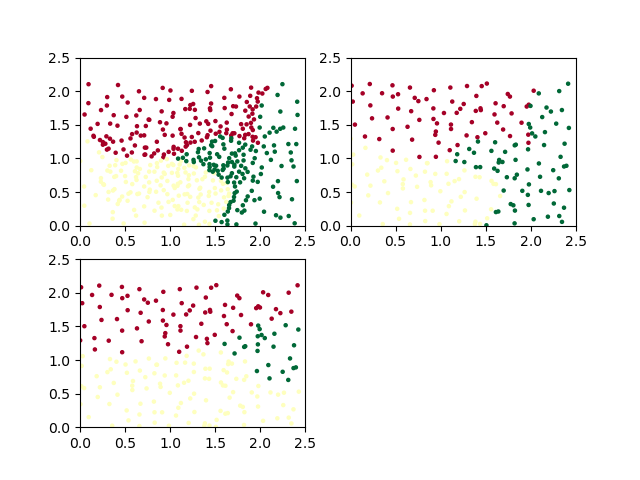
\includegraphics[width=5.5cm]{insets_2-10-6-3_0.02_100_73.81_05.070578.png}}
		\subfigure[2-10-6-3 0.02 1000 87.14 24.342106]{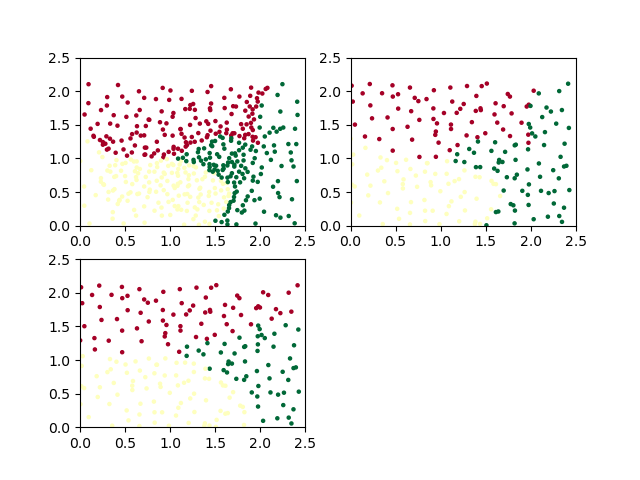
\includegraphics[width=5.5cm]{insets_2-10-6-3_0.02_1000_87.14_24.342106.png}}
		\subfigure[2-10-6-3 0.02 10000 89.05 4:02.436815] %子图片标题
		{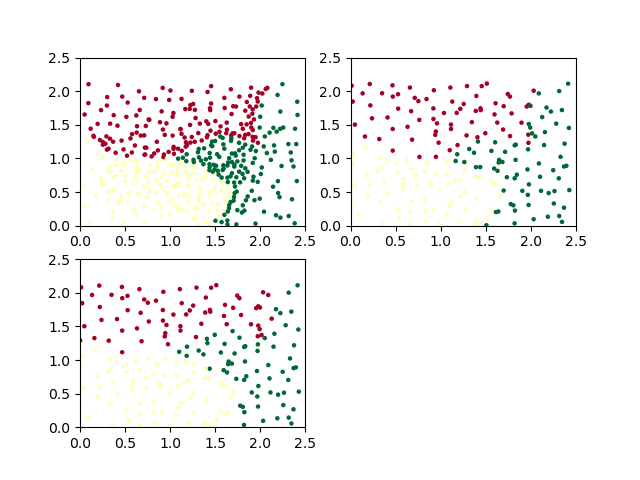
\includegraphics[width=5.5cm]{insets_2-10-6-3_0.02_10000_89.05_4:02.436815.png}} %[图片大小]{图片路径}
		\caption{昆虫数据集不同迭代次数的比较} %图片标题
		\label{fig:1}  %图片交叉引用时的标签
	\end{figure}

    \begin{figure}[htbp]
		\centering
		\subfigure[learningrate=0.01]{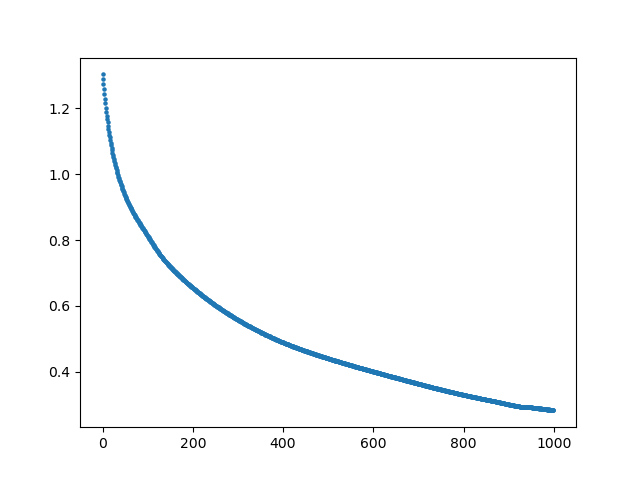
\includegraphics[width=5.5cm]{insets_2-10-6-3_0.01.png}}
		\subfigure[learningrate=0.05]{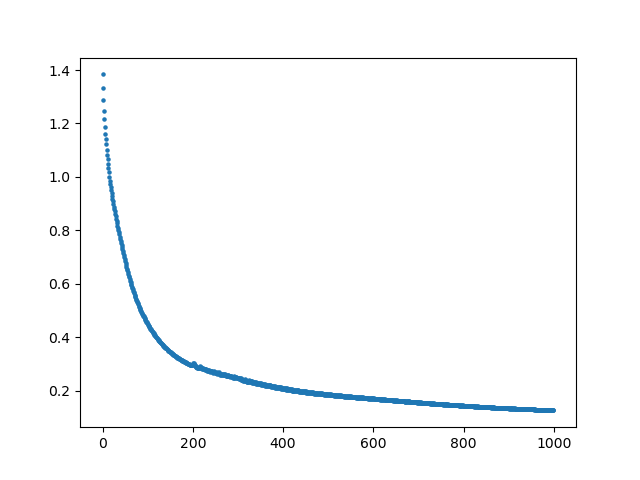
\includegraphics[width=5.5cm]{insets_2-10-6-3_0.05.png}}
		\subfigure[learningrate=0.1] %子图片标题
		{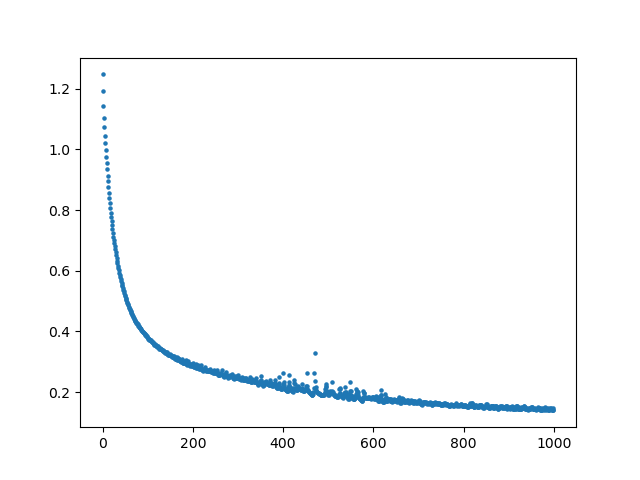
\includegraphics[width=5.5cm]{insets_2-10-6-3_0.1.png}} %[图片大小]{图片路径}
		\caption{昆虫数据集2-10-6-3网络结构\ loss-迭代次数\ 图像} %图片标题
		\label{fig:1}  %图片交叉引用时的标签
	\end{figure}

    \begin{figure}[htbp]
		\centering
		\subfigure[2-10-3结构 准确率85.24\%]{\includegraphics[width=8cm]{insets_2-10-3_0.05_1000_85.24\%.png}}
		\subfigure[2-10-6-3结构 准确率89.05\%]{\includegraphics[width=8cm]{insets_2-10-6-3_0.05_1000_90\%_20.847109.png}}
		\caption{昆虫数据集2-10-6-3网络结构\ loss-迭代次数\ 图像} %图片标题
		\label{fig:1}  %图片交叉引用时的标签
	\end{figure}

    \begin{figure}[htbp]
    	\centering %居中
    	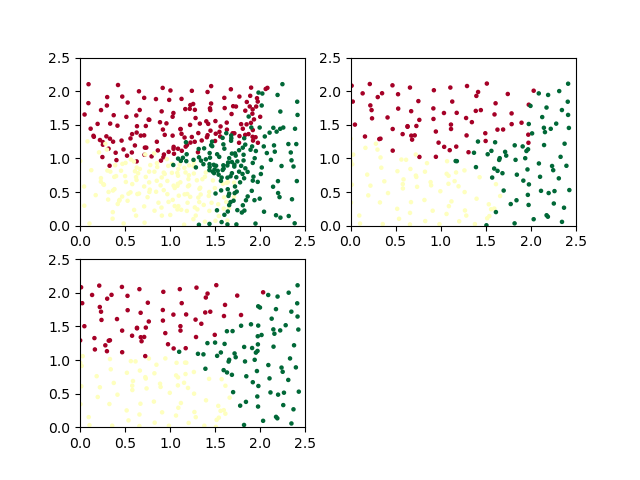
\includegraphics[scale=0.5]{insets2_89.52.png}
    	\caption{有噪声insets数据集结果\  准确率为89.52\%}
    \end{figure}

    \begin{figure}[htbp]
		\centering
		\subfigure[无噪声Points数据集测试结果 准确率94.21\%]{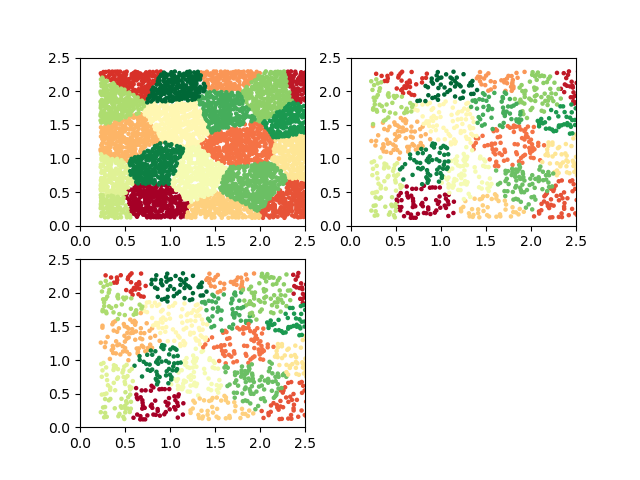
\includegraphics[width=8cm]{points_94.21.png}}
		\subfigure[有噪声Points数据集测试结果 准确率91.61\%]{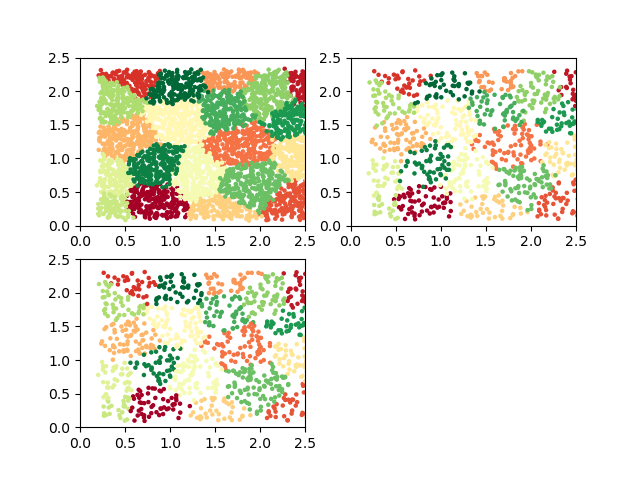
\includegraphics[width=8cm]{points2_91.61.png}}
		\caption{points数据集测试结果图像} %图片标题
		\label{fig:1}  %图片交叉引用时的标签
	\end{figure}

    \begin{figure}[htbp]
		\centering
		\subfigure[激活函数为relu]{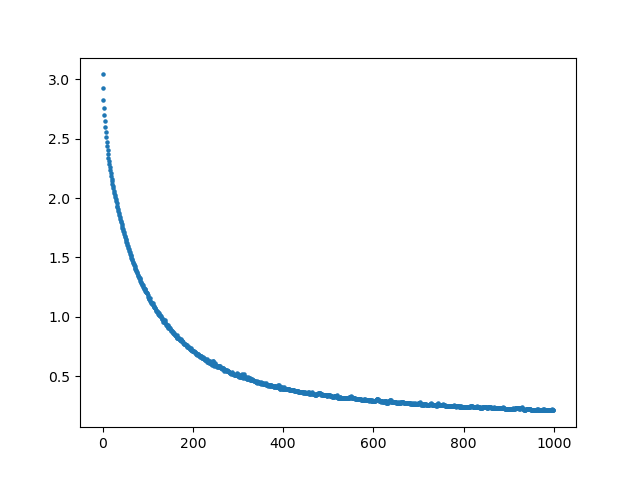
\includegraphics[width=5cm]{points_relu.png}} 
		\subfigure[激活函数为sigmoid]{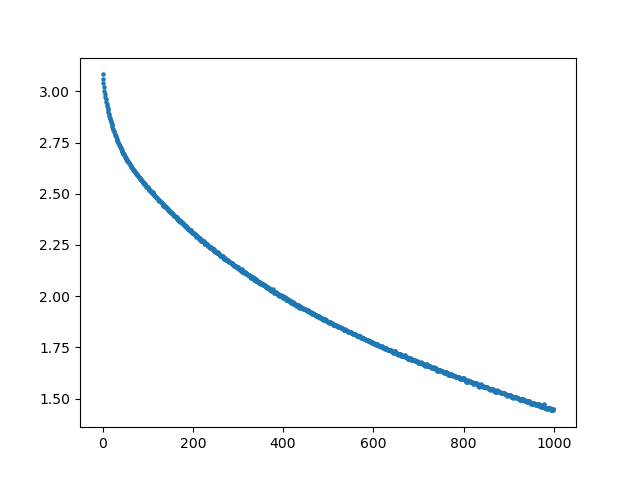
\includegraphics[width=5cm]{points_sigmoid.png}}
		\\ %换行
		\centering
		\subfigure[激活函数为tanh]{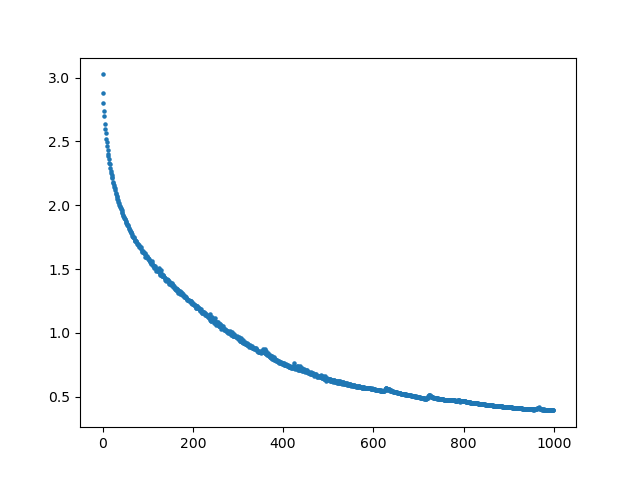
\includegraphics[width=5cm]{points_tanh.png}} 
		\subfigure[激活函数为elu]{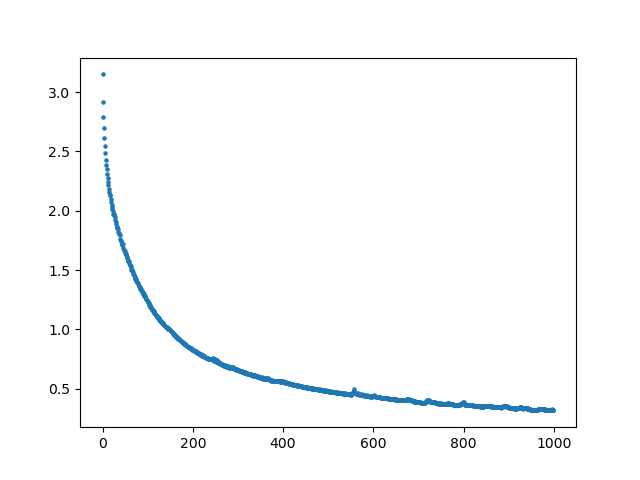
\includegraphics[width=5cm]{points_elu.png}}
		
		\caption{不同激活函数收敛速度的比较} %图片标题
	\end{figure}

 \setcounter{section}{8}
\section*{\centerline{八、结论}}
    由上述结果可知以下结论:
    \begin{itemize}
        \item [1)]
        不同的网络结构会影响结果,网络越复杂越容易发现数据中的隐藏规则,但相对的也会牺牲一些时间效率,我们需要找到两者之间的平衡点。
        一般像本次作业中一样的简单数据并不需要过于复杂的网络结构,1到2层隐藏层即可。
        \item [2)]
        通过不同数量级的迭代次数对比,可以得到最佳的迭代次数,避免迭代次数过少还未收敛就结束了程序,
        同时也减少了时间的浪费,接近收敛时就结束迭代,不会进行过多的无用迭代。也可以从loss-迭代次数图像中找到最佳迭代次数。
        \item [3)]
        学习速率过高会导致无法精确找到局部最优解,导致结果效果差。
        而学习速率过低会使得收敛时间变长,找到局部最优解会浪费大量时间,所以需要找到合适的学习速率平衡精确度与时间开销。
        \item [4)]
        不同激活函数对收敛速度有所影响,应选取合适的激活函数,ReLU函数就是个很好的函数。
        
    \end{itemize}  

 \setcounter{section}{9}
\section*{\centerline{九、问题与优化}}
\begin{itemize}
    \item [1)]
    网络传播过程中要进行正规化(normalization),这样能大幅提升梯度下降速率。
    经测试不进行正规化的复杂网络(多层网络)收敛速度极慢,基本需要10000到100000次迭代才能基本有效;
    而如果在传递过程中进行正规化,基本迭代次数在1000左右就能得到很好的效果。
    \item [2)]
    画出loss-迭代次数曲线可以很好的找到最佳迭代次数,也可直接设置一个指定的误差常量,
    在Loss值不小于该常数时进行迭代。
\end{itemize}  

\setcounter{section}{10}
\section*{\centerline{十、代码及程序说明}}
    本次提交代码有两份.py文件分别为NN.py,NNnew.py文件。NN.py为初始版本,能实现单隐藏层网络。
    NNnew.py为优化后的版本,对代码结构进行了一定优化(设置全局变量、对代码根据逻辑进行重排等)。
    如要进行测试请使用NNnew.py文件。该文件有全局变量learningRate,iterations,它们可以设置学习速率与迭代次数。
    文件上方有文件路径,可直接修改以对不同数据集进行测试。
    测试者也可以通过修改网络结构测试不同的网络,只需要修改”Net()“括号中的数据。

    程序还会动态显示数据集训练过程,将数据训练可视化。程序运行过程中输出的图片意义在结果说明中已经介绍就不再赘述。

\bibliographystyle{ieeetr}
\bibliography{refer}

\end{document}